\section{GUI}
\label{sec:gui}
The GUI contains following tabs:
\begin{itemize}
  \item \textbf{Enrollment} \\

    \begin{figure}[H]
      \centering
      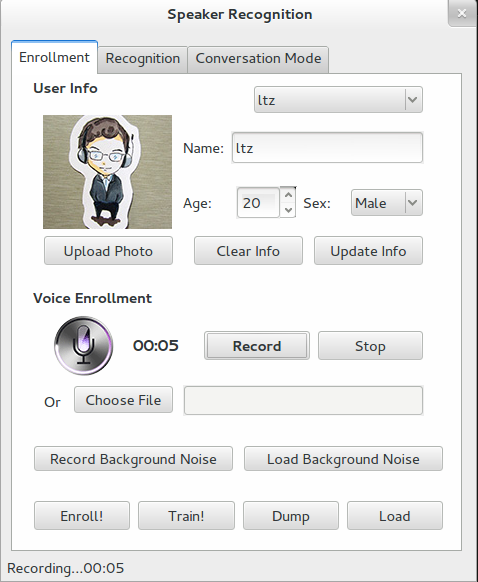
\includegraphics[width=0.8\textwidth]{img/enrollment.png}
    \end{figure}

    A new user may start his or her first step by clicking the
    tab Enrollment. New users could provide personal information
    such as name, sex, and age. then upload personal avatar to
    build up their own data. Experienced users can choose from
    the userlist and update their infomation.

    Next the user needs to provide a piece of utterance for
    the enrollment and training process.

    There are two ways to enroll a user:
    \begin{itemize}
      \item \textbf{Enroll by Recording}
        Click Record and start talking while click Stop to stop
        and save.There is no limit of the content of the utterance,
        whileit is highly recommended that the user speaks long enough
        to provide sufficient message for the enrollment.

      \item \textbf{Enroll from Wav Files}
        User can upload a pre-recorded voice of a speaker.(*.wav recommended)
        The systemaccepts the voice given and the enrollment of a speaker is done.
    \end{itemize}

    The user can train, dump or load his/her voice features after enrollment.

  \item \textbf{Recognition of a user} \\
    \begin{figure}[H]
      \centering
      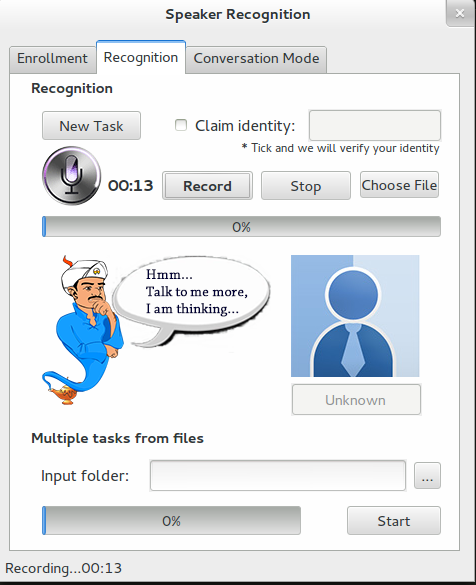
\includegraphics[width=0.8\textwidth]{img/recognition.png}
    \end{figure}

    An user present  can record a piece of utterance, or provide a wav file,
    then the system will tell who the person is and show his/her avatar.
    Recognition of multiple pre-recorded files can be done as well, the result will be printed in the command line.

  \item \textbf{Conversation Recognition Mode} \\
    \begin{figure}[H]
      \centering
      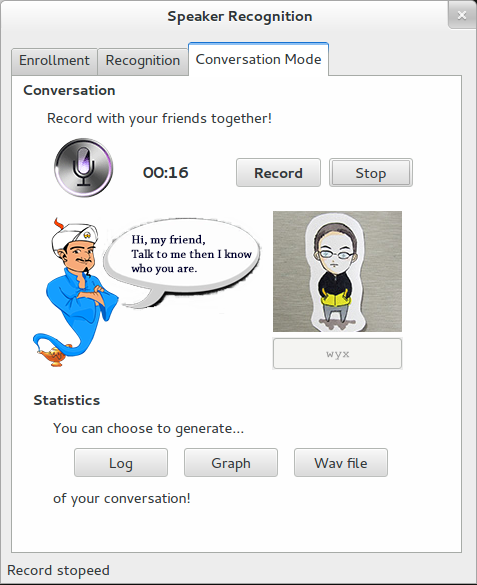
\includegraphics[width=0.8\textwidth]{img/conversation.png}
      \caption{\label{fig:}}
    \end{figure}

    In Conversation Recognition mode, multiple users can have conversations
    together near the microphone. Same recording procedure as above.
    The system will continuously collect voice data, and determine
    who is speaking right now. Current speaker's anvatar will show up
    in screen; otherwise the name will be shown.

    We can show a \textbf{Conversation flow graph} to visualize the recognition.
    A timeline of the conversation will be shown by a number of
    talking-clouds joining together, with start time, stop time
    and users' avatars labeled. The avatar of the talking person will also be larger than the others.
    Different users are displayed with different colors in the timeline,
    and the timeline flows to the left dynamically just as time elapses.
    \begin{figure}[H]
      \centering
      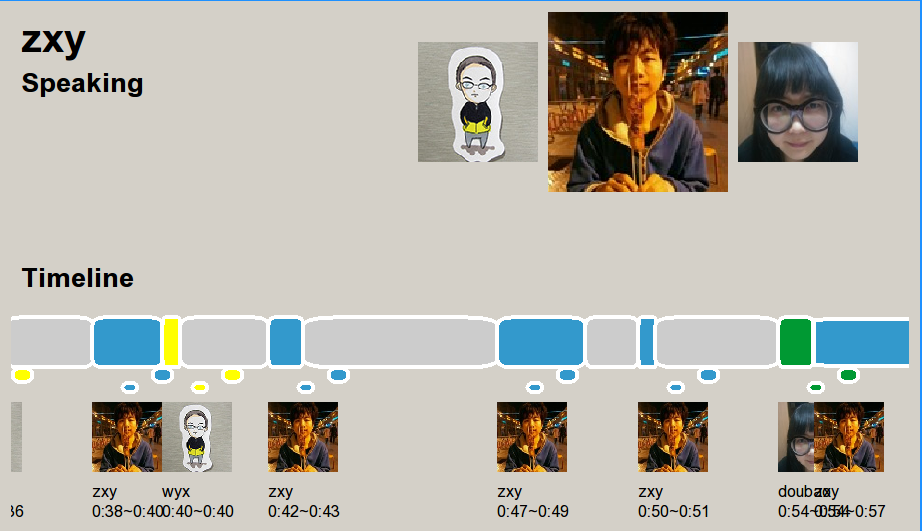
\includegraphics[width=0.8\textwidth]{img/gui-graph.png}
    \end{figure}

\end{itemize}
